\documentclass[border=4pt]{standalone}
% Shared style for the workflow figures (standalone TikZ, compiled to PDF).
\usepackage[T1]{fontenc}
\usepackage[scaled=0.95]{helvet}
\renewcommand{\familydefault}{\sfdefault}
\usepackage{amsmath,amssymb}
\usepackage{xcolor}
\usepackage{tikz}
\usetikzlibrary{arrows.meta,positioning,calc,fit,backgrounds,shapes.misc,shapes.geometric}

\definecolor{cBlue}{HTML}{2B6CB0}
\definecolor{cTeal}{HTML}{1C8C8C}
\definecolor{cGreen}{HTML}{2F855A}
\definecolor{cPurple}{HTML}{6B46C1}
\definecolor{cOrange}{HTML}{C05621}
\definecolor{cRed}{HTML}{C53030}
\definecolor{cGray}{HTML}{4A5568}
\definecolor{cInk}{HTML}{1A202C}

\tikzset{
  cardbody/.style={rectangle, rounded corners=3pt, line width=0.9pt, align=left,
                   font=\scriptsize\color{cInk}, inner xsep=5pt, inner ysep=5pt},
  cardhead/.style={rectangle, rounded corners=3pt, align=left, text=white,
                   font=\footnotesize, inner xsep=4pt, inner ysep=3.5pt},
  numc/.style={circle, line width=0.9pt, inner sep=0pt, minimum size=5.2mm,
               font=\footnotesize\bfseries},
  flow/.style={-{Stealth[length=2.6mm,width=2.2mm]}, line width=1.3pt, color=cGray},
  loop/.style={-{Stealth[length=2.4mm,width=2mm]}, line width=1.1pt, dashed, color=cRed},
  tag/.style={rectangle, rounded corners=2pt, font=\scriptsize\bfseries, inner sep=2.5pt},
  note/.style={font=\scriptsize\itshape, color=cGray, align=center},
  band/.style={rectangle, rounded corners=6pt, line width=0.8pt, inner sep=7pt},
}

% \card{name}{position}{colour}{number}{title}{body}{width}{body height}
\newcommand{\card}[8]{%
  \node[cardbody, draw=#3, fill=#3!5, text width=#7, minimum height=#8, anchor=north]
       (#1) at (#2) {#6};
  \node[cardhead, fill=#3, text width=#7, anchor=south, yshift=-1.5pt] (#1h) at (#1.north) {\hspace*{4.2mm}\textbf{#5}};
  \node[numc, fill=white, draw=#3, text=#3] at ([xshift=1pt]#1h.west) {#4};
}
\newcommand{\bul}{\textcolor{cGray}{\textbullet}~}

\tikzset{dec/.style={diamond, aspect=2.2, draw=cGray, line width=0.9pt, fill=white, font=\scriptsize\bfseries, inner sep=1.5pt, align=center},
         act/.style={rectangle, rounded corners=3pt, draw=#1, fill=#1!8, line width=0.9pt, font=\scriptsize, align=center, text width=2.6cm, minimum height=0.95cm}}
\begin{document}
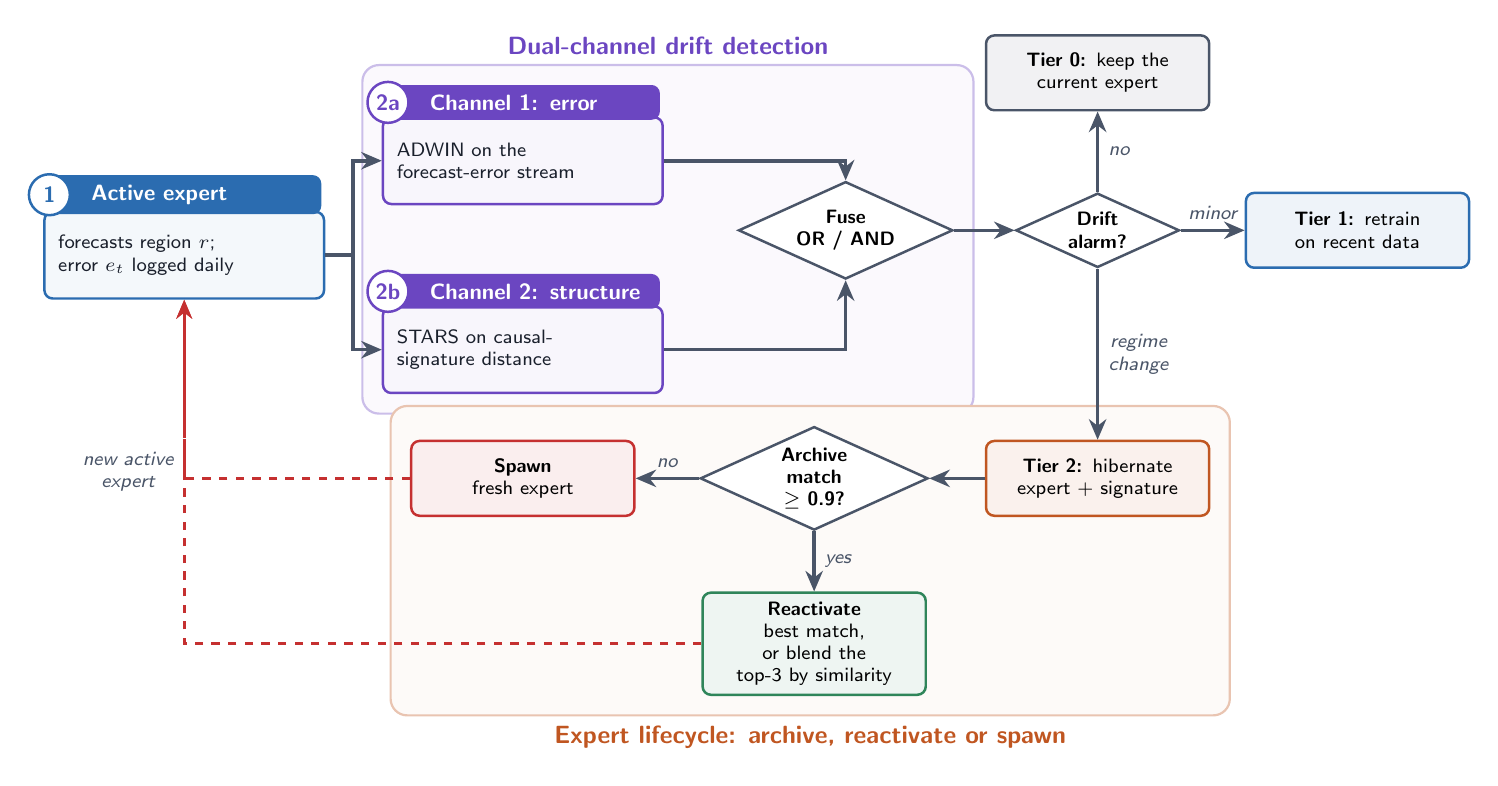
\begin{tikzpicture}
\def\W{3.2cm}
\card{ex}{0,0}{cBlue}{1}{Active expert}{forecasts region $r$;\\error $e_t$ logged daily}{\W}{1.1cm}
\card{c1}{4.3,1.2}{cPurple}{2a}{Channel 1: error}{ADWIN on the\\forecast-error stream}{\W}{1.1cm}
\card{c2}{4.3,-1.2}{cPurple}{2b}{Channel 2: structure}{STARS on causal-\\signature distance}{\W}{1.1cm}
\node[dec] (fuse) at (8.4,-0.25) {Fuse\\OR / AND};
\draw[flow] (ex.east) -- ++(0.35,0) |- (c1.west);
\draw[flow] (ex.east) -- ++(0.35,0) |- (c2.west);
\draw[flow] (c1.east) -| (fuse.north);
\draw[flow] (c2.east) -| (fuse.south);
\node[dec] (alarm) at (11.6,-0.25) {Drift\\alarm?};
\draw[flow] (fuse) -- (alarm);
\node[act=cGray] (t0) at (11.6,1.75) {\textbf{Tier 0:} keep the\\current expert};
\draw[flow] (alarm) -- node[note, right]{no} (t0);
\node[act=cBlue] (t1) at (14.9,-0.25) {\textbf{Tier 1:} retrain\\on recent data};
\draw[flow] (alarm) -- node[note, above]{minor} (t1);
\node[act=cOrange] (arch) at (11.6,-3.4) {\textbf{Tier 2:} hibernate\\expert + signature};
\draw[flow] (alarm) -- node[note, right]{regime\\change} (arch);
\node[dec] (match) at (8.0,-3.4) {Archive\\match\\$\ge$ 0.9?};
\draw[flow] (arch) -- (match);
\node[act=cGreen] (react) at (8.0,-5.5) {\textbf{Reactivate}\\best match, or blend the\\top-3 by similarity};
\node[act=cRed] (spawn) at (4.3,-3.4) {\textbf{Spawn}\\fresh expert};
\draw[flow] (match) -- node[note, right]{yes} (react);
\draw[flow] (match) -- node[note, above]{no} (spawn);
\draw[loop] (react.west) -| node[note, pos=0.75, left]{new active\\expert} (ex.south);
\draw[loop] (spawn.west) -| (ex.south);
\begin{scope}[on background layer]
\node[band, draw=cPurple!35, fill=cPurple!3, fit=(c1h)(c2)(fuse), label={[font=\small\bfseries\color{cPurple}]above:Dual-channel drift detection}] {};
\node[band, draw=cOrange!35, fill=cOrange!3, fit=(arch)(match)(react)(spawn), label={[font=\small\bfseries\color{cOrange}]below:Expert lifecycle: archive, reactivate or spawn}] {};
\end{scope}
\end{tikzpicture}
\end{document}
